\section{IBE and AKE}

This section aims to describe the IBE and AKE schemes developed as part of the SAFEcrypto project from an implementation perspective. It should be noted that both schemes are almost identical.

\subsection{Key Generation}

IBE and AKE rely upon the algorithm in Figure \ref{fig:ibe_keygen} to generate the public key \textit{h} and \textit{Master Secret Key \textbf{B}}. In IBE the \textit{Extract} function (see Figure \ref{fig:ibe_extract}) is detached from Key Generation as it is required to derive a secret key for each user from the master key, whilst it is incorporated into AKE's key generation function as it effectively has only one user \textit{id} (see Figure \ref{fig:ake_digital_signature}).

The key generation function is quite involved. The principle operations involve repeated trials of the randomly generated keys \textit{(f, g)} with Extended GCD and GCD functions until co-prime relationships have been found. An added complexity of this step is the need to compute the GCD's using large integer arithmetic in order to obtain an integer GCD and Bezout coefficients.

\begin{figure}[H]
\centering
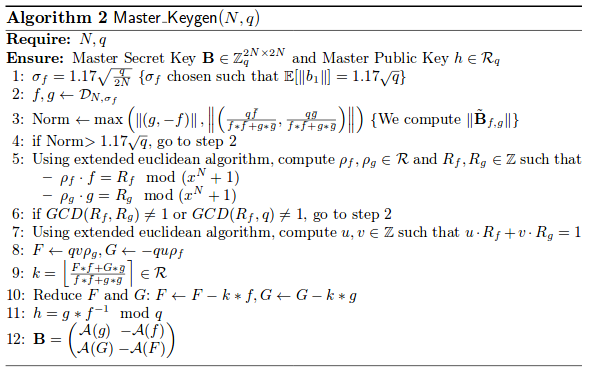
\includegraphics[width=11cm]{ibe_keygen.png}
\caption{IBE KeyGen}
\label{fig:ibe_keygen}
\end{figure}

\begin{figure}[H]
\centering
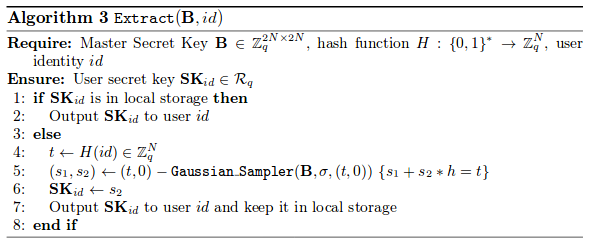
\includegraphics[width=11cm]{ibe_extract.png}
\caption{IBE Extract}
\label{fig:ibe_extract}
\end{figure}

\begin{figure}[H]
\centering
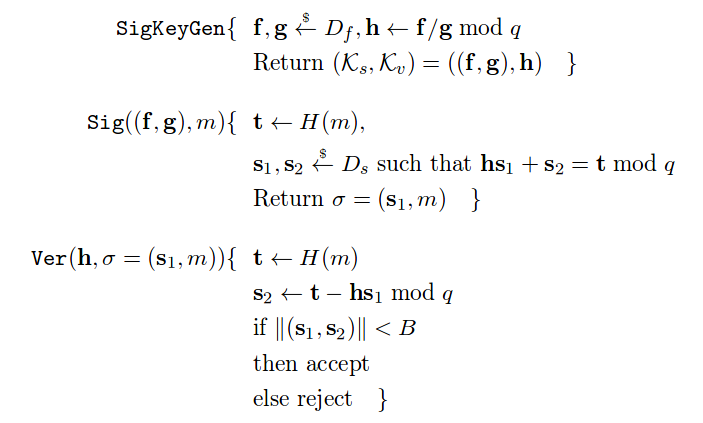
\includegraphics[width=9cm]{ake_hash_and_sign.png}
\caption{Whole is less... Digital Signature Scheme}
\label{fig:ake_digital_signature}
\end{figure}

\subsection{IBE Encrypt and Decrypt}

The IBE encrypt and decrypt operations involve mapping binary bits onto the lattice and recovering them - in a similar manner to the RLWE encryption scheme. It should be noted that this scheme uses large modulus values to reduce the failure probability of the encryption operation - therefore decryption failures should be expected at a negligible rate during any testing of the scheme.

\begin{figure}[H]
\centering
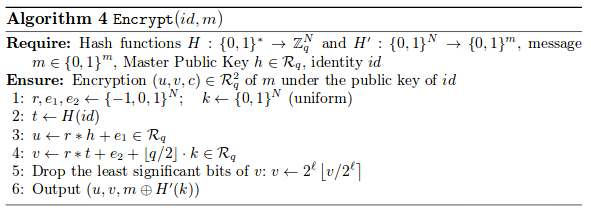
\includegraphics[width=14cm]{ibe_encrypt.png}
\caption{IBE Encrypt}
\label{fig:ibe_encrypt}
\end{figure}

\begin{figure}[H]
\centering
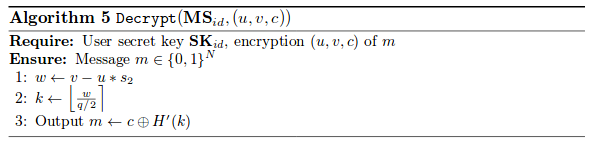
\includegraphics[width=14cm]{ibe_decrypt.png}
\caption{IBE Decrypt}
\label{fig:ibe_decrypt}
\end{figure}

\subsection{Extract and Signing}

AKE signing is almost identical to IBE extract, both requiring Gaussian Sampling over a lattice.

\subsection{AKE Signatures with Message Recovery}

AKE also defines a \textit{Signature with Message Recovery} scheme (see Figure \ref {fig:ake_signature_with_recovery}) that can be used to produce smaller signatures at the cost of more CPU cycles. Instead of sending the signature as $(s_1, m)$ and recovering $s_2$, it is instead transmitted as $(s_1, s_2)$ and the message $m$ is recovered by the verifier.

\begin{figure}[H]
\centering
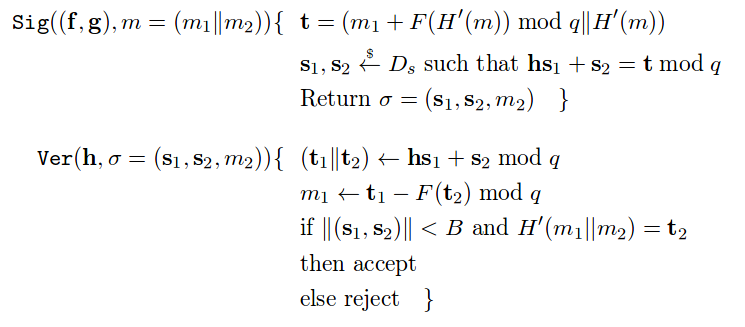
\includegraphics[width=11cm]{ake_with_message_recovery.png}
\caption{Whole is less... Digital Signature Scheme with Message Recovery}
\label{fig:ake_signature_with_recovery}
\end{figure}


\subsection{Software Implementation}

The generic AKE scheme shown in Figure \ref{fig:generic_ake} indicates that the signature keys are typically generated once whilst the KEM keys are generated on a per-session basis. Therefore the complexity of AKE \textit{SigKeyGen} should not be a burden as it can effectively be treated as an off-line computation. Real performance gains in a system will be achieved by optimising the regularly used \textit{Sign, Verify, KEMKeyGen, Encapsulate} and \textit{Decapsulate} operations. Similarly for IBE, the regularly used \textit{Extract, Encrypt} and \textit{Decrypt} functions should be the focus of optimisation.

\begin{figure}[H]
\centering
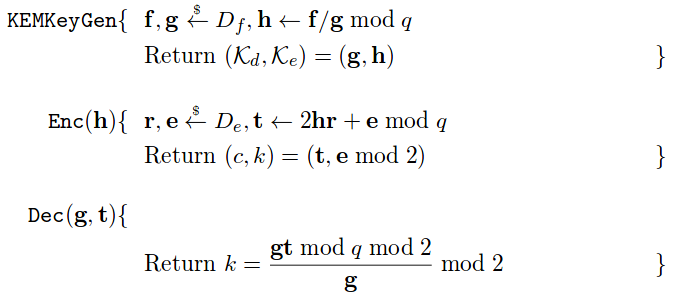
\includegraphics[width=9cm]{ake_kem.png}
\caption{AKE KEM}
\label{fig:ake_kem}
\end{figure}

\begin{figure}[H]
\centering
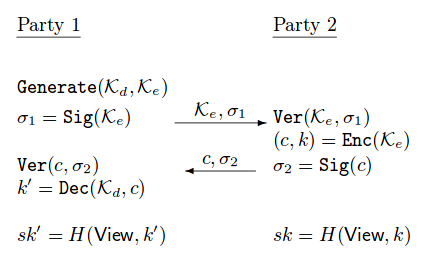
\includegraphics[width=7cm]{generic_ake.png}
\caption{A Generic AKE Construction from a KEM and a Digital Signature}
\label{fig:generic_ake}
\end{figure}

The main areas of work that are foreseen in implementing both IBE and AKE within the SAFEcrypto library are the following:

\begin{enumerate}[1]
\item A generic implementation of the IBE \textit{Master\_Keygen} function to be used by both IBE and AKE.
\begin{enumerate}[a]
\item Big integer arithmetic functions (add/sub, multiply, divide, GCD) [currently using GMP, libtommath has been added to the build system].
\item XGCD with integer polynomial coefficients (NTL and FLINT have this function and can be used as a reference).
\end{enumerate}
\item Implementing a discrete Gaussian Sampling scheme over a lattice using the polynomial basis \textit{\textbf{B}}, i.e. IBE Extract and AKE SigKeyGen.
\item Verifying the correctness of the already implemented AKE KEM as one of the parameter sets appears to be incorrect.
\item Acceleration of the Whole KEM scheme, in particular inversion modulo 2 used in \textit{KEMKeyGen}.
\item Re-factoring the RLWE Encryption encrypt/decrypt source code for IBE encrypt/decrypt.
\end{enumerate}
